\begin{document}

\title{An Overview of the Bandwidth Managemet Module}
\section{Bandwidth Management System}
In PeerSim there are no mechanisms to simulate network layer, this means that we need to implement a mechanism for bandwidth management as in real life. A very simple technique could be the one where both upload and download bandwidth are assigned to a connection when it starts and do not change for the whole connection time so there are no bandwidth fluctuations.

We want to use asymmetric bandwidth, and to reproduce bandwidth fluctuations during transmissions, we want that each transmission tries to use as much resource as possible and each peer manages its bandwidth resources as better as possible. This means that if at a certain time there is unused upload bandwidth, the peer tries to speed-up its upload transmission using this free bandwidth. We assume that peers know or can estimate their bandwidth with some techniques.

In order to implement this mechanism, each peer has to store a connections Table for both upload and download bandwidth. This table collects connection elements that contains the amount of bandwidth from initial to end time. We talk about max-min fairness share mechanism, which inspire our bandwidth management mechanism.

\subsection{Max-Min Fairness Mechanism}\label{sub:max-min-fair-mechanism}
We try to simulate real scenerios, where peers have a well-known limited amount of resources: computational resource, storage space and bandwidth. We focus our attention on bandwidth management mechanism in order to simulate transmissions more accurately.

The problem of dividing a scarce resource among a set of consumer, where each consumer has an equal right to the resource and someone asks more resources than other, was widely analyzed in computer science. 

A shared technique widely adopted in practice is called \textit{max-min fairness}. This technique allocates resources to consumer in order of increasing demand and evenly distributed unused resources to those consumers that need more. This technique grants that no consumer obtains more resources than its demand and consumer with unsatisfied demand receives and equal share of the resource.

More formally, consider a set of consumer $1, 2, \ldots, n$ that demand a certain amount of resource $r_{1},r_{2},\ldots,r_{n}$ where  
$r_{1} \leq r_{2} \leq\ldots\leq r_{n}$ and $C$ is the quantity of the resource to share. We initially assign $C/n$ of the resource to the smallest demand $r_{1}$, this quantity may be more than demand, the exceed quantity is added to residual resource and the process continue.

Applying max-min fairness in our simulations is very difficult because it needs to retrieve and modify all the events added in the queue of the simulator, and when an element is modified it causes other modifications. Consider a peer that starts to upload a chunk to a target peer using all bandwidth, after few seconds, this peer receives a pull request, now it accepts this request and should divide the upload bandwidth between the two uploads using max-min fairness criteria, shifting finish time of the first transmission, so we have to search this event of the first transmission in the queue of the simulator, modifying the time at which it will be scheduled, the resource used by sender and also by receiver. After this modifications, the receiver could have more download bandwidth to redistribute among its download transmissions, this means that it can go faster and all the corresponding upload peers will be modified in the queue of the simulator.

Replicate this mechanism in our simulations means uses ``all'' computational resources only to maintain consistent the queue of the simulator, and we want to simulate our protocol not simulate this mechanism.

\subsection{Simulation of Max-min Fairness Mechanism}
We adopt a mechanism for bandwidth management that is inspired to max-min fairness, this mechanism allocates as much resource as possible to each transmission, analyzing connections Table of each involved peer and when a transmission ends, it releases the resources on both side that will be assigned to other transmissions. We propose two example to better explain our mechanism, where the limited resources are upload and download bandwidth respectively, then we compare this mechanism to the transmission mechanism proposed in section \ref{Interleave event-based}.

In the first example (figure \ref{max-min-fairness-upload}), peer $A$ has an upload bandwidth of $128000\;bps$ and some of its upload is busy because it is satisfying a pull started at time $t_0$ which ends at time $t_2$ from peer $B$. Peer $B$ uses all its free available download bandwidth $100000\;bps$, the residual download of peer $B$ is $0$ while the residual upload of peer $A$ is $28000\;bps$. At time $t_{1}$ peer $A$ tries to push data to peer $C$, this transmission start at $28000\;bps$ from $t_{1}$ to $t_{2}$ and when first transmission ends at time $t_{2}$ peer $A$ tries to go faster, peer $C$ has available download bandwidth and transmission speed increase from $28000\;bps$ to $128000\;bps$.
\begin{figure}[ht]
\centering
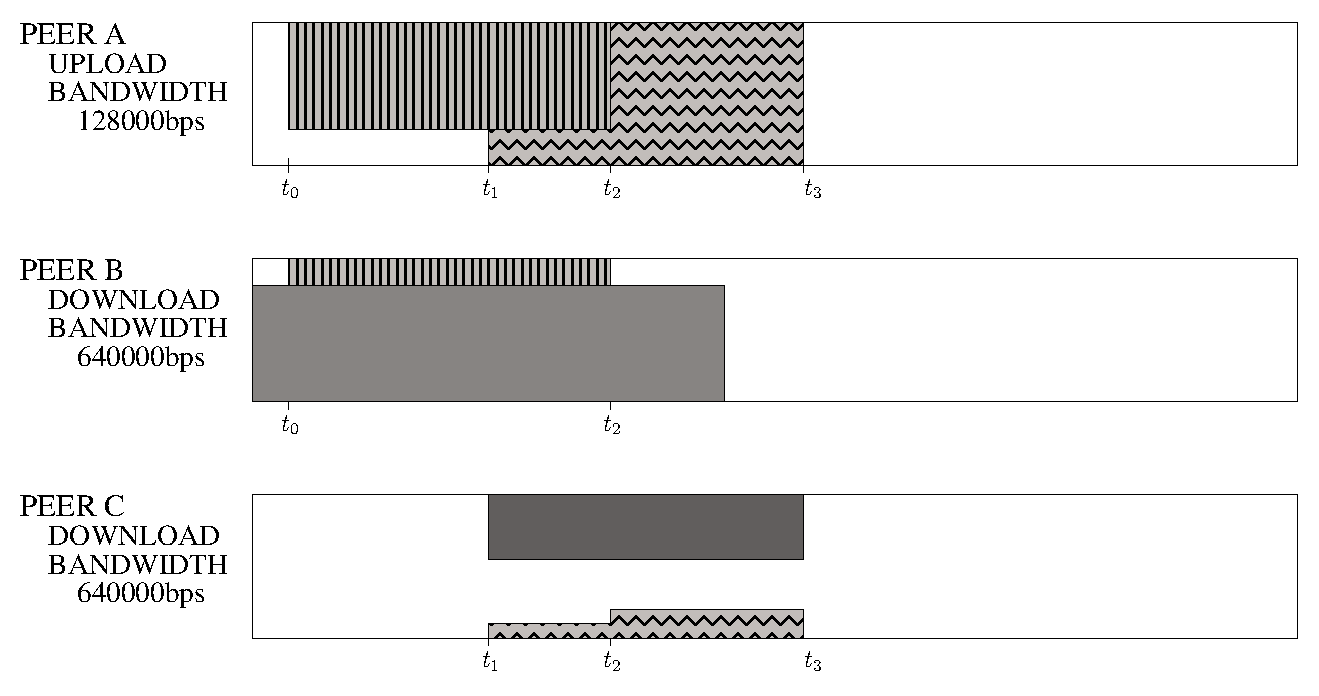
\includegraphics[width=\textwidth]{img/max-min-fairness-upload.eps}
\caption{Bandwidth management mechanism used - upload.}
\label{max-min-fairness-upload}
\end{figure}

If peer $A$ receives some requests to use its upload bandwidth between $t_{1}$ and $t_{3}$, it refuses this transmissions because it has no upload bandwidth until $t_{3}$, and start to accept upload transmission after $t_{3}$.

In the second example (figure \ref{max-min-fairness-download}) we have peer $A$ that has started to push data at time $t_{0}$ to peer $B$ until time $t_{2}$ at maximum speed that is $512000\;bps$. At time $t_{1}$ peer $C$ starts a transmission with peer $B$ pushing data, transmission speed is $128000\;bps$ until time $t_{2}$ where download resources of peer $B$ become available and transmission speed-up to $256000\;bps$ finishing at time $t_{3}$.
\begin{figure}[ht]
\centering
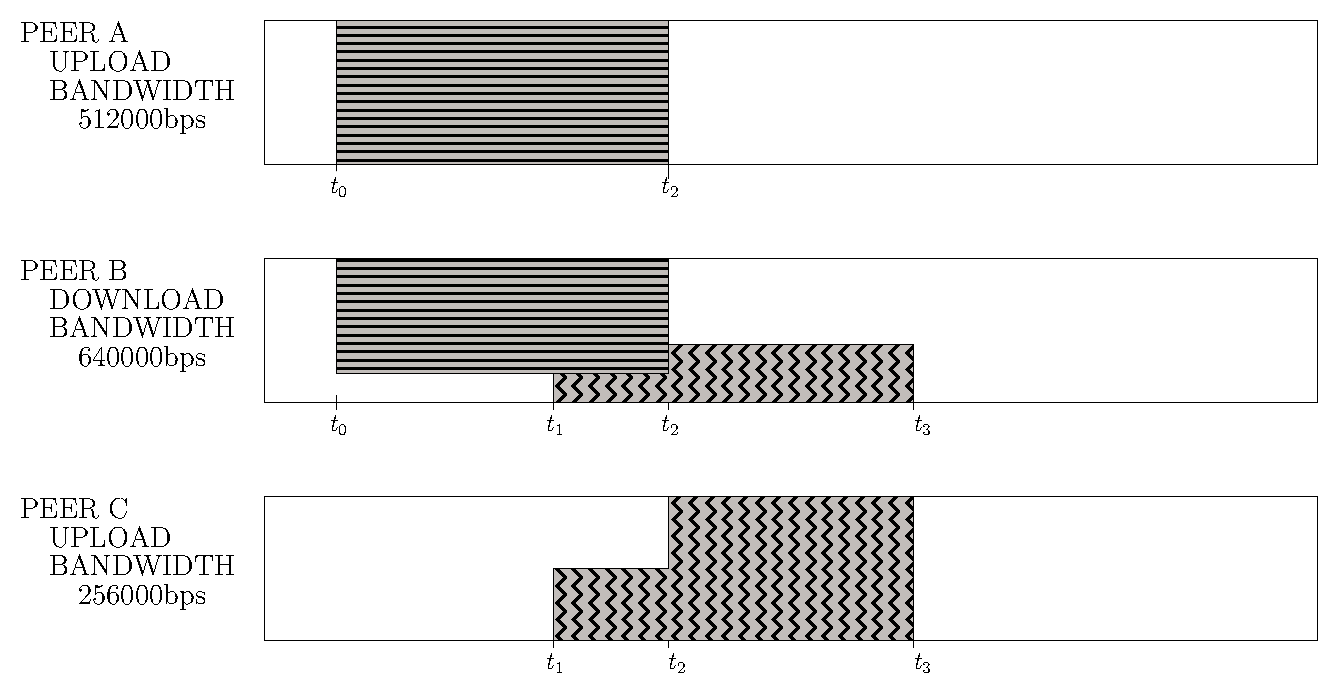
\includegraphics[width=\textwidth]{img/max-min-fairness-download.eps}
\caption{Bandwidth management mechanism used - download.}
\label{max-min-fairness-download}
\end{figure}

\subsection{Comparing Bandwidth Management Mechanisms}
In the simple bandwidth management mechanism a node uploads data to a target node, using the same amount of bandwidth which is the minimum between upload and download bandwidth available, and the transmission time is
\begin{displaymath}
tx\;time = \frac{data\;size}{min(sender.upload, receiver.downlod)}
\end{displaymath}

The bandwidth used for the transmission is subtracted to both peers and is restored when transmission ends. The transmission bandwidth is fixed to a certain value for the entire transmission time, this means that transmissions cannot speed-up if resources are release by other transmissions as shown in Figure \ref{normalized-problem-one}.

Peer $A$ starts a transmission to peer $B$ with bandwidth $512000\;bps$ then peer $C$ start a transmission with peer $B$ with bandwidth $128000\;bps$, with this technique the second transmission is performed at $128000\;bps$ until ends while with our bandwidth management mechanism, sender speed-up transmission to $256000\;bps$ at time $t_{2}$ because peer $C$ terminates transmission with $A$ and corresponding download bandwidth at peer $C$ become available, our mechanism uses all available resources like a real bandwidth management technique.
\begin{figure}[ht]
\centering
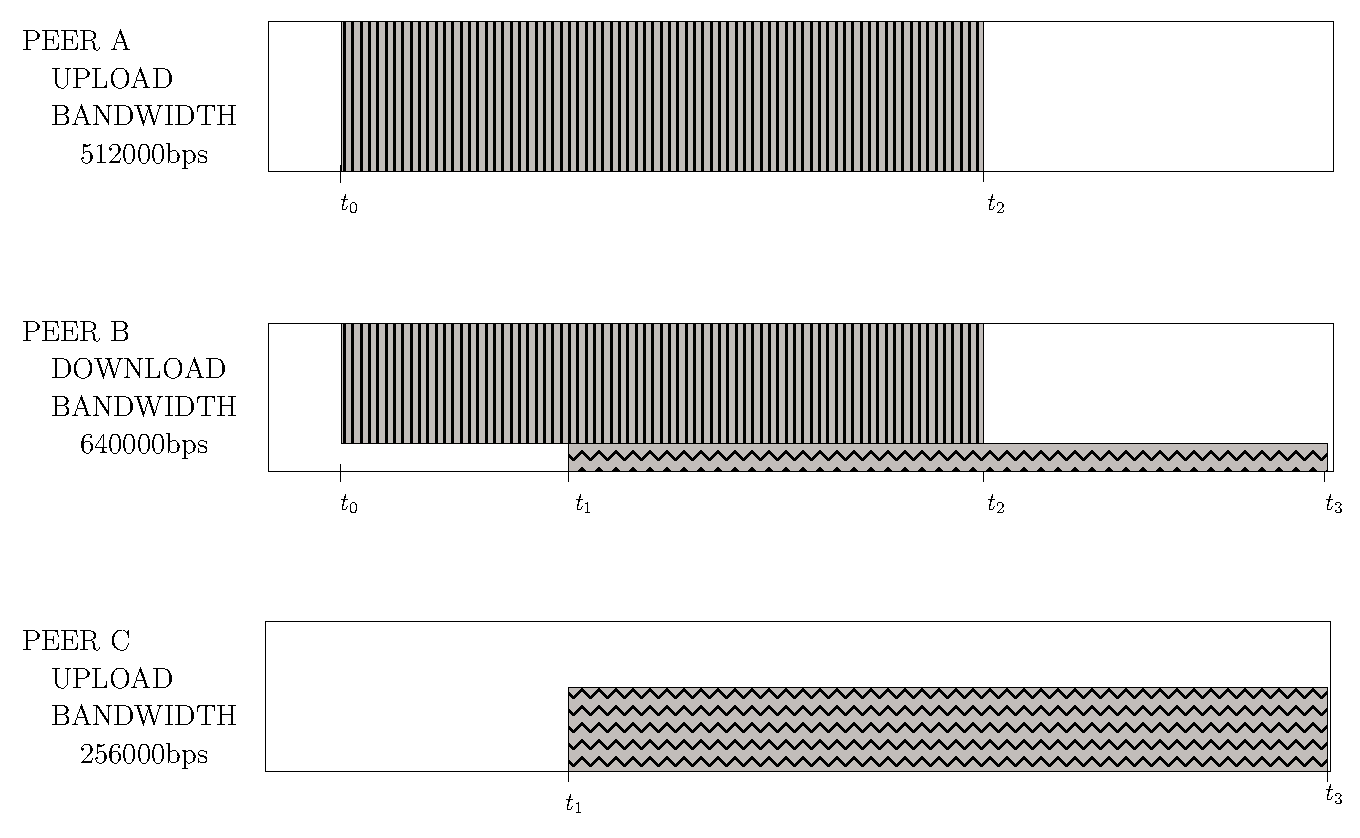
\includegraphics[width=\textwidth]{img/simple-bandwidth-management-problem.eps}
\caption{Simple bandwidth management mechanism.}
\label{normalized-problem-one}
\end{figure}

\subsection{Problem Discovered}
Upload bandwidth is the bottleneck for file distribution systems. Each nodes maintain two connections tables: one for upload and one for download bandwidth. The mechanism that we used is very simple and the numbers of updates that affect the these table is very low, this means that computational power used to compute the time in which update the bandwidth is limited.

Using our mechanism, when a nodes has many active connections in the same table, some problems could happen. A peer can start a transmission with a target peer which has only a small amount of complementary bandwidth. The peer supposes that the scarce resource at the target peer will be released later, when the corresponding transmission that keep busy the scarce resource ends, and this transmission could be speed-up.

The problem is how long is the time interval in which the transmission go slow: It may be very long, occupying a small amount of both upload and download bandwidth for a lot of time and then may speed-up. The target node can either accept or refuse the transmission, basing its answer on amount of available resources in the time it receives the message, and also in the future using its connections tables.

An example is reported in Figure \ref{max-min-fairness-problem}, where peer $B$ starts a transmission with peer $A$ at time $t_{0}$ until $t_{3}$, using its download bandwidth. Then peer $C$ starts an upload transmission with peer $B$ at time $t_1$ which could speed-up at time $t_3$, but the upload bandwidth of peer $C$ become available later, at time $t_{4}$. At time $t_2$ peer $D$ starts a transmission with peer $B$ which accepts, but this transmission is very slow between $t_{2}$ and $t_{3}$.

In order to avoid this situations in which a transmissions may take a lot of time at slow speed, peers could refuse these transmission if the amount of free resources is less then a certain threshold, set up appropriately. In our example peer $B$ will refuse the transmission with peer $D$, that could transmit data to another peer faster.

Now we will show simulative results for Interleave event-based model where the source has the same resources of the other peers, no messages are lost and no peers leave or join the network during chunk distribution.
\begin{figure}[ht]
\centering
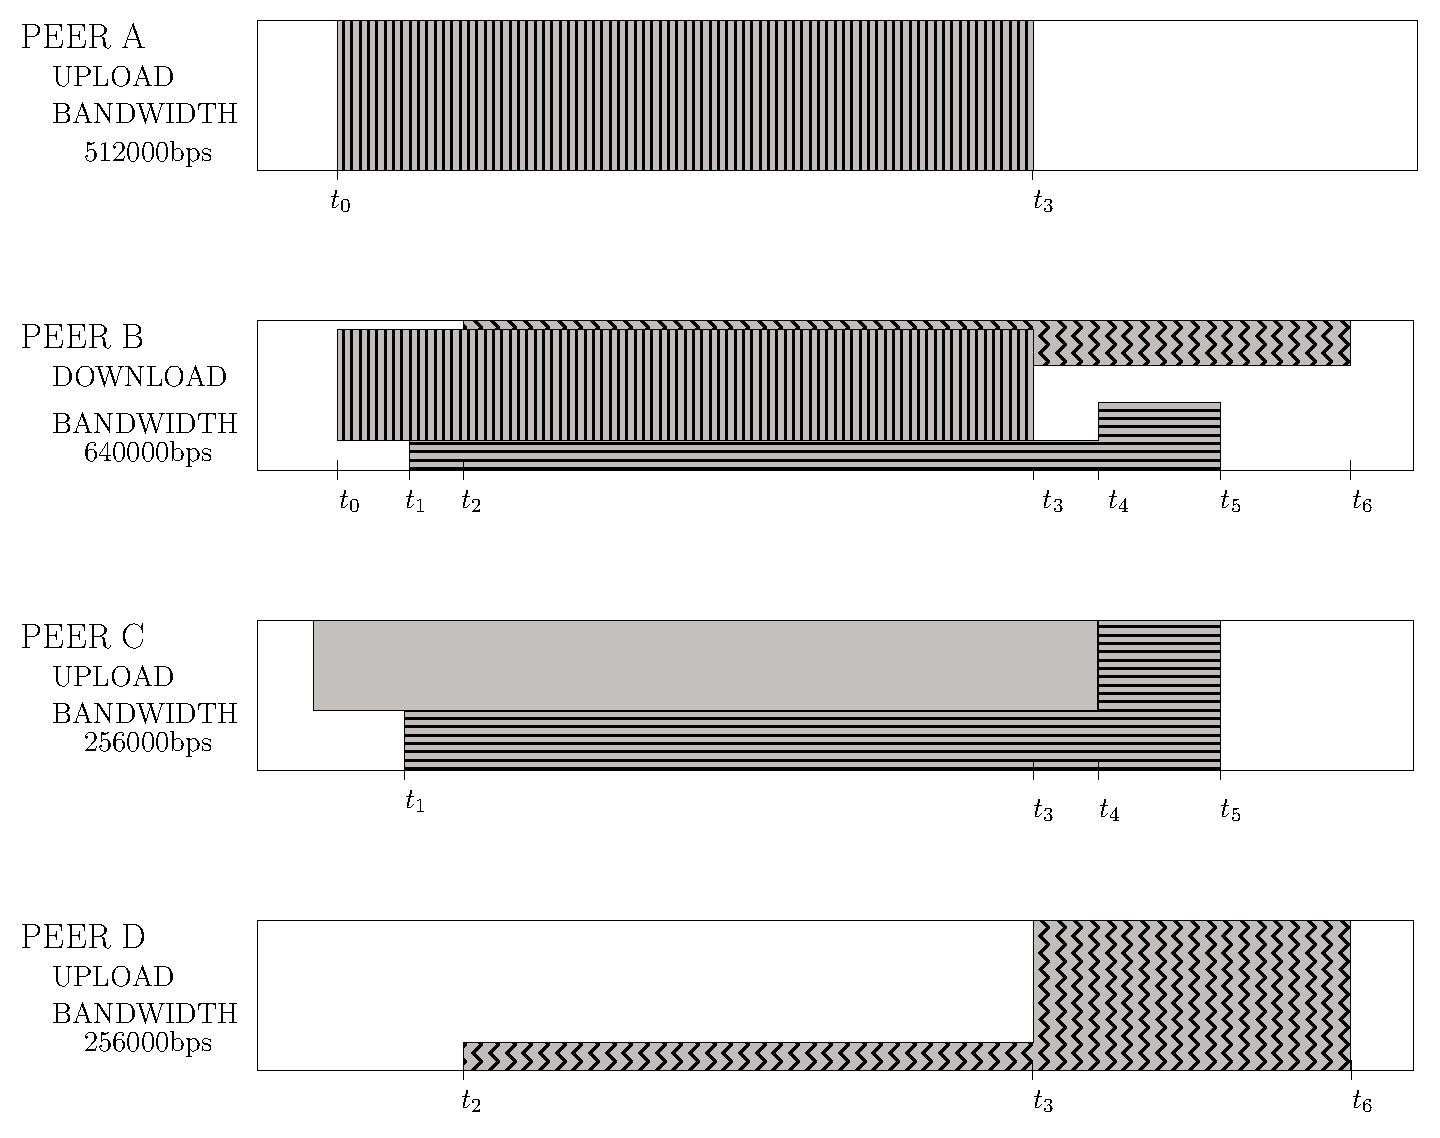
\includegraphics[width=\textwidth]{img/max-min-fairness-problem.eps}
\caption{Problem with our Bandwidth management mechanism.}
\label{max-min-fairness-problem}
\end{figure}
\end{document}
